% Theoretical background
%\clearpage % Uncomment if needed to force a page break before the chapter
\vspace{21.5pt}
\chapter{Teoreettinen tausta}

Jotta voidaan löytää pragmaattinen näkökulma funktionaaliseen ohjelmointiin, on käsiteltävä funktionaalisen ohjelmoinnin teoreettisia perusteita ja keskeisiä käsitteitä.

Tarkastellaan joukko-opin sovelluksia ohjelmoinnissa käytännön tasolla. Sivutaan kategoriateorian osuutta funktionaalisessa ohjelmoinnissa ilman syvällistä paneutumista yksityiskohtiin.

Tutkitaan, miten nämä käsitteet integroituvat moderniin ohjelmistokehitykseen, kuten TypeScriptin käyttöön.

On tärkeää huomata, että tämän insinöörityön tavoitteena ei ole tarjota kattavaa opasta kaikkeen funktionaaliseen ohjelmointiin, vaan keskittyä valittuihin aihealueisiin, jotka tukevat työn pääteemoja ja osoittavat, miten teoreettiset käsitteet voidaan soveltaa käytännön ohjelmointihaasteisiin.

Valitut aihealueet pyritään avaamaan \glsdisp{language_agnostic}{kieliagnostisesti}, ja myös JavaScript- sekä TypeScript-ekosysteemien näkökulmista.

Lopulta näillä tiedoilla voidaan lähteä tutkimaan miten funktionaalisen ohjelmoinnin käytänteet näkyvät hyödyllisesti (tai haitallisesti) ohjelmistoprojekteissa.

Tässä teoriaosuudessa pyritään sisältö mielenkiintoisena ja liimaamalla käsitteet yhdeksi kokonaisuudeksi. Teoriaan pyritään tuomaan konkretiaa erilaisilla esimerkeillä.

\section{Funktionaalinen ohjelmointi}

Funktionaalinen ohjelmointi on ohjelmointiparadigma, jonka juuret ulottuvat 1930-luvulle ja lambda-kalkyylin kehitykseen. Lähestymistapa korostaa funktioiden käyttöä perusyksikköinä ja pyrkii välttämään muuttuvia tiloja sekä sivuvaikutuksia. Funktionaalisen ohjelmoinnin keskeisiä käsitteitä ovat \glsdisp{pure_function}{puhtaat funktiot}, \glsdisp{higher_order_function}{korkeamman asteen funktiot}, \glsdisp{composed_function}{yhdistetyt funktiot}, sekä \gls{declarative_programming}. Funktiot ovat funktionaalisessa ohjelmoinnissa tosiaankin keskiössä. \citep{Tan2004,computerphile_lambda}

\subsection{Työn nimeämiskäytänteet}

Ohjelmoidessa funktionaalista ohjelmakoodia nimeämiskäytänteet ovat yhtä vaikeita kuin aina. Tässä insinöörityössä käytetään Haskell-ohjelmoijien keskuudessa näkyviä nimeämiskäytänteitä, jossa käytetään lyhyitä ja \textquote{intuitiivisia} nimiä funktioille ja muuttujille. Esimerkiksi:

\begin{itemize}
    \item x: Yleisesti käytetty muuttuja tai parametri, joka edustaa arvoa, jota funktiot käsittelevät. Jos näkyvyysalalla on muita funktioita, niitä nimetään usein aakkosjärjestyksessä x:stä eteenpäin (x, y, z).
    \item xs: Muuttuja, joka edustaa useita arvoja (useita x-kirjaimia). Usein sisältää listan arvoista, mutta tietorakenteen tietäminen ei ole merkittävää.
    \item f: Yksittäinen funktio, jota voidaan käyttää käsittelemään arvoja. Jos näkyvyysalalla on muita funktioita, niitä nimetään usein aakkosjärjestyksessä f:stä eteenpäin (f, g, h, i...).
    \item fs: Muuttuja, joka edustaa useita funktioita (useita f-kirjaimia). Usein sisältää listan funktioista, mutta tietorakenteen tietäminen ei ole merkittävää.
\end{itemize}

Esimerkkejä käytänteiden käytöstä:

\begin{code}
    \begin{minted}{javascript}
const map    = f => xs => xs.map(f)
const either = f => g => x => f(x) || g(x)
const max    = x => y => x > y ? x : y
const pipe   = fs => x => fs.reduce((acc, f) => f(acc), x)
\end{minted}
    \caption{Esimerkkejä insinöörityössä käytettävistä nimeämiskäytänteistä.}
    \label{code:javascript_naming_convention_example}
\end{code}

\subsection{Puhtaat funktiot}

Funktionaalisessa ohjelmoinnissa \glsdisp{pure_function}{puhtaat funktiot} ovat funktioita, jotka poikkeuksetta aina palauttavat samalle syötteelle saman arvon. Funktion puhtauden voi päätellä siitä, jos sen voisi teoreettisesti korvata hakutaulukolla. \citep{feldman_fp_pragmatists}

Puhtaista funktioista hyötyy siten, että niitä voi käyttää uudelleen ja uudelleen kontekstista riippumatta. Puhtailla funktioilla voi rakentaa järjestelmäriippumattomia kirjastoja.

Puhtaiden funktioiden perusta on matematiikassa. Jos matemaattinen funktio $f(x) = x+2$ esimerkiksi ei aina palauttaisi samalle $x$ arvolle samaa palautusarvoa, mitä hyötyä funktiosta edes olisi? Toivottavasti $2 + 2$ tulee aina olemaan $4$.

\subsection{Kombinaattorit}

Funktionaalinen ohjelmointi mahdollistaa koodin uudelleenkäytettävyyden. Lambda-kalkyylin perustein joka ikisien ongelman voi purkaa pieniksi funktioiksi \cite{BlellochHarper2015}. Lambda-kalkyylin voi ajatella olevan esoteerinen ohjelmointikieli. Sen voi kuitenkin myös ottaa osaksi ohjelmoijan työkalupakkia missä tahansa ohjelmointikielessä, joka kohtelee funktioita ensiluokkaisina, eli siten, että niitä voi käyttää muuttujina (Koodiesimerkki \ref{code:javascript_combinators}).

Jos kombinaattoreille haluaa etsiä vastaavanlaista määritelmää olio-ohjelmoinnin termeistä, voisi niitä ajatella olevan perustavanlaatuisia suunittelumalleja.

\begin{code}
    \begin{minted}{javascript}
const identity      = x => x
const constant      = x => y => x
const apply         = f => x => f (x)
const thrush        = x => f => f (x)
const duplication   = f => x => f (x) (x)
const flip          = f => y => x => f (x) (y)
const compose       = f => g => x => f (g (x)) 
const substitution  = f => g => x => f (x) (g (x))
\end{minted}
    \caption{Yleiset kombinaattorit esitettynä JavaScriptissä \cite{javascript_combinators}. Kombinaattoreilla voi esittää lambda-kalkyyliä, ja ohjelmoida Turing-vahvoja ohjelmia.}
    \label{code:javascript_combinators}
\end{code}

Kombinaattorit näyttävät uhkaavilta ja raa'assa muodossaan niiden hyötyarvoa voi olla hankala havaita. Niiden käyttämistä voi kuitenkin perustella niiden perustavanlaatuisten ja kieliagnostisien ominaisuuksien takia. Ohjelmoidessa funktionaalisesti ei kombinaattoreita kuitenkaan tarvitse paljoa ajatella. Niitä tulee kirjoittamaan varmasti vähintään vahingossa, sillä niitä vaaditaan funktioita pyörittäessä \cite{javascript_combinators}. Kuitenkin on hyvä tiedostaa käytössä olevat rakennuspalikat, ja millä nimellä etsiä niistä tietoa tarvittaessa.

\subsection{Yhdistefunktiot ja niiden vahva merkitys}

Usein funktionaalista ohjelmointia mainostaessa puhutaan funktioiden puhtauden ja datan muuttumattomuuden olevan paradigman oleellisinta. Kuitenkin samaan aikaan juuri datan muuttumattomuus ja tilattomuus koetaan paradigman suureksi kompastuskiveksi \cite{cantarella_fp_haitat,is_reduce_bad,vakil2016}.

On tärkeää huomata, että kaiken ei tarvitse olla täysin puhdasta ja muuttumatonta, kunhan ne osat, joissa funktionaalista ohjelmointia hyödynnetään, pysyvät ennustettavina ja hallittavina.

\Glspl{composed_function} ovat loistava tapa kirjoittaa selkeää ja modulaarista koodia. Parasta on, että kaiken ei tarvitse olla pelkkiä funktioita: voi hyvin kirjoittaa myös olio-ohjelmointityylillä ja silti hyödyntää yhdistefunktioita logiikan selkeyttämiseksi ja yksinkertaistamiseksi.

Loppujen lopuksi funktionaalisen ohjelmoinnin perusta on funktioissa ja niiden yhdistämisessä. Datan muuttumattomuus ja sivuvaikutuksettomuus on vain esivaatimus funktioiden ennustettavuudelle.

\Gls{composed_function} tarkoittaa yksinkertaisesti kahden, tai useamman, funktion yhdistämistä siten, että yhden funktion tulos syötetään seuraavalle. Esimerkiksi koodiesimerkin \ref{code:javascript_manual_composition} funktio $h$ on funktioiden $f$ ja $g$ yhdiste. Ajaessa funktio $h$, suoritetaan ensin $g$, jonka palautusarvo annetaan funktiolle $f$. Kaksi funktiota yhdistämällä on saatu yksi uusi funktio.

\begin{code}
    \begin{minted}{javascript}
const f = x => 2 * x

const g = x => x + 3

const h = x => f(g(x))
\end{minted}
    \caption{JavaScript-esimerkki yhdistetystä funktiosta h ilman pipe tai compose funktiota}
    \label{code:javascript_manual_composition}
\end{code}

Funktionaalisissa ohjelmointikielissä yhdistettyjä funktioita pystyy usein kirjoittamaan käyttäen kieleen sisäänrakennettuja operaattoreja, joilla funktioiden yhdistäminen on helppoa ja suoraan osana ohjelmointikieltä \cite{fsharpcomposition,haskellcomposition}.
JavaScriptissä ei ole vastaavanlaista sisäänrakennettua operaattoria.
(Vaikkakin sellainen on kehitteillä \cite{tc39_pipeline_operator}.)
Operaattorin voi kuitenkin kirjoittaa funktiona helposti osaksi mitä vain koodikantaa (Koodiesimerkki \ref{code:javascript_pipe_composition}).

\begin{code}
    \begin{minted}{javascript}
const pipe    = f => g => x => g(f(x))
const compose = f => g => x => f(g(x))

const h = pipe(f)(g)
// tai vaihtoehtoisesti
const h = compose(g)(f)
\end{minted}
    \caption{JavaScript-esimerkki funktiokompositiosta pipe ja compose funktioilla}
    \label{code:javascript_pipe_composition}
\end{code}

Voi olla mielenkiinoista huomata, että koodiesimerkin \mintinline{javascript}{compose} löytyy myös koodiesimerkin \ref{code:javascript_combinators} tunnetuista yleisistä kombinaattoreista.

Koodiesimerkissä \ref{code:javascript_pipe_composition} on näytettynä kaksi eri tapaa yhdistää funktioita: \mintinline{javascript}{pipe} ja \mintinline{javascript}{compose}. Käytännössä tapojen ainoa ero on se, kummasta suunnasta funktiot suoritetaan. \mintinline{javascript}{compose} on lähempänä yhdistettyjen funktioiden matemaattisia perusteita, kun taas \mintinline{javascript}{pipe} on usein helpompi lukea, sillä se suoritetaan yleisessä lukemissuunnassa, eli vasemmalta oikealle, tai ylhäältä alas. Tulevissa koodiesimerkeissä tullaan suosimaan funktioiden yhdistämistä käyttäen \mintinline{javascript}{pipe}-funktiota \mintinline{javascript}{compose}-funktion sijaan. \citep{whyprefercompose}

Esimerkin \ref{code:javascript_pipe_composition} \mintinline{javascript}{pipe} ja \mintinline{javascript}{compose} toimivat vain kahdelle funktiolle kerrallaan. Tämä tapa seuraa lambda-kalkyyliä \cite{computerphile_lambda}. Ohjelmointikielestä riippuen voi kuitenkin olla mieluisaa kirjoittaa funktiot niin, että ne tukevat suoraan mielivaltaista määrää funktioita.

JavaScriptissä näin voi tehdä esimerkiksi hyödyntämällä Array-tietorakennetta (Koodiesimerkki \ref{code:javascript_better_pipe}).

\begin{code}
    \begin{minted}{javascript}
const pipe    = fs => x => fs.reduce((acc, f) => f(acc), x)
const compose = fs => x => fs.reduceRight((acc, f) => f(acc), x)

const f = x => x + 1
const g = x => x * 2
const h = x => x - 3

const i = pipe([f, g, h])
i(5) // (((5 + 1) * 2) - 3) = 9
// tai vaihtoehtoisesti 
const i = compose([h, g, f])
i(5) // (((5 + 1) * 2) - 3) = 9
\end{minted}
    \caption{JavaScript-esimerkki yhdistettyjen funktioiden luomisesta käyttäen \mintinline{javascript}{reduce} ja \mintinline{javascript}{reduceRight} funktioita}
    \label{code:javascript_better_pipe}
\end{code}

Mikä tästä sitten tekee loistavaa? Se, että ohjelmointi on kerrankin oikeasti kuin LEGO palikoilla leikkimistä (Koodiesimerkki \ref{code:javascript_composition_example}).

\begin{code}
    \begin{minted}{javascript}
const pipe     = fs => x => fs.reduce((acc, func) => func(acc), x)
const multiply = x => y => x * y
const add      = x => y => x + y
const filter   = f => xs => xs.filter(f)
const map      = f => xs => xs.map(f)
const isEven   = x => x % 2 === 0

const rejectOdds   = filter(isEven)
const multiplyBy10 = multiply(10)

const pipeline = pipe([rejectOdds, map(multiplyBy10)])

pipeline([1, 2, 3, 4]) // [20, 40]
\end{minted}
    \caption{Käytännöllinen JavaScript-esimerkki yhdistettyjen funktioiden käyttämisestä laskutoimituksiin}
    \label{code:javascript_composition_example}
\end{code}

Esimerkissä näytetyt funktiot ovat hyvin yksinkertaisia. Kuitenkin ne ovat täysin uudelleenkäytettäviä. Jos totuttautuu käyttämään joitain funktioita kaikissa projekteissa, voi huomata koodin kirjoittamisen tehokkuuden ja johdonmukaisuuden kasvavan.

\section{Joukko-oppi}
Joukko-oppi on matematiikan haara, joka tutkii joukkojen ominaisuuksia ja niiden välisiä suhteita. Ohjelmoinnissa joukko-oppi ilmenee yksinkertaisimmin joukko-tietorakenteiden kautta, jotka mahdollistavat uniikkien alkioiden käsittelyn tehokkaasti ja ilmaisuvoimaisesti \cite{mdn_set,mdn_set_methods}. On myös luotu ohjelmointikieli, joka perustuu kokonaan joukko-oppiin \cite{SETL_SET_LANGUAGE}.


Tämä osa pyrkii kirjoittamaan matemaattisista käsitteistä pragmaattisesti ja mahdollisesti suurelti yksinkertaistaen. Ajatuksena on, että ylemmän tason ajattelumalli välittyisi tekstissä tarkkojen määritelmien sijasta.


\subsection{Joukko-tietorakenne}

Ohjelmoinnissa joukko-tietorakennetta käytetään hyvin laajasti, ja sen merkitys on keskeinen monissa ohjelmointikielissä, kuten Pythonissa, Javassa ja JavaScriptissä. Joukko-tietorakenne mahdollistaa alkioiden tallentamisen ilman duplikaatteja. Sen operaatiot, kuten unioni, leikkaus ja erotus, ovat suoraan peräisin matemaattisesta joukko-opista. Joukko-tietorakenteen tehokkuus ja yksinkertaisuus tekevät siitä tehokkaan työkalun monenlaisissa sovelluksissa. \citep{mdn_set,ecma_spec}

Joukko-tietorakenne kuvaa joukko-opin joukkoa. Joukko-tietorakenteessa säilytetään kokoelma uniikkeja alkioita. Joukko-tietorakenne on ohjelmoinnissa mieluinen työkalu sen tehokkuuden ansiosta. \citep{ecma_spec}

Kokemusten mukaan ohjelmoija ei usein mieti joukko-tietorakennetta matemaattisista lähtökohdista. Tästä kuitenkin voisi olla hyötyä, sillä Joukko-opin periaatteiden ymmärtäminen ja soveltaminen ohjelmoinnissa ei ainoastaan tehostuskeino, vaan myös laajentaa näkemystä siitä, miten abstraktit matemaattiset konseptit voidaan muuttaa konkreettisiksi työkaluiksi. Tämä yhdistelmä tarjoaa ohjelmoijille sekä teoreettisen että käytännöllisen perustan, joka on arvokas monissa erilaisissa sovelluksissa ja ongelmanratkaisutilanteissa \cite{bartosz_category_for_progamers}.

\subsection{Funktiot joukoista toisiin}
Kun ohjelmoinnissa pohditaan joukko-opin hyödyntämistä, kehittyy \glsdisp{language_agnostic}{kieliriippumaton} kyky kirjoittaa koodia. Kun miettii, mitä ylipäätään voi laskea, pääsee ohjelmoinnissa omalle abstraktille tasolle. \citep{Tan2004,BlellochHarper2015}


Matemaattisesti joukkojen välille voidaan tehdä kuvauksia, tai toisin sanoen funktioita. Merkintä funktiosta, joka \textquote{muuttaa} joukon $A$ joukoksi $B$, on esimerkiksi yksinkertaisesti $A \to B$ \cite{mellin2005joukkooppi}. Funktio muuttaa minkä tahansa joukon $A$ alkion joksikin joukon $B$ alkioksi.

Funktionaalisessa ohjelmoinnissa puhtaiden funktioiden voidaan ajatella aina olevan rinnastettaessa jonkin joukon muutokseksi johonkin toiseen joukkoon (Esimerkkikoodi \ref{code:ts_set_example}) \cite{bartosz_category_for_progamers}. (Toisaalta funktioiden argumentit ja palautusarvot ovat aina joukkoja riippumatta siitä onko funktio puhdas vai ei. Ei-puhtaat funktiot eivät kuitenkaan välttämättä luo yksikäsitteisiä muutoksia joukkojen alkioille.)

\begin{code}
    \begin{minted}{typescript}
type SetA = 'a' | 'b' | 'c'
type SetB = 1 | 2 | 3
const aToB = (a: SetA): SetB => {
    switch (a) {
        case 'a': return 1
        case 'b': return 2
        case 'c': return 3
    }
}  
\end{minted}
    \caption{Havainnollistava funktio, joka muuttaa joukon A, \{a,b,c\}, joukoksi B, \{1, 2, 3\}}
    \label{code:ts_set_example}
\end{code}



Tarkastellaan konkreettisempaa esimerkkiä lähtien koodiesimerkistä \ref{code:ts_set_theory_3}.

\begin{code}
    \begin{minted}{typescript}
const divide = (x:number) => (y:number) => x / y
\end{minted}
    \caption{Funktio, joka jakaa numeron toisella}
    \label{code:ts_set_theory_3}
\end{code}



Funktio ottaa kaksi numeroa, ja jakaa ensimmäisen toisella. Argumentit on tyypitetty JavaScript-numeroiksi. Jos kyseistä funktiota haluaa käyttää, ohjelmoijan tulisi tietää, että nollalla ei voi jakaa, ja että jos niin kuitenkin tehdään, JavaScript palauttaa arvon \mintinline{javascript}|Infinity| (tai erityisemmässä tapauksessa \mintinline{javascript}|NaN|) (Koodiesimerkki \ref{code:ts_division}).


\begin{code}
    \begin{minted}{typescript}
console.log(1/0)  // Infinity
console.log(1/-0) // -Infinity
console.log(0/0)  // NaN
\end{minted}
    \caption{Jakamisoperaattorin toiminta JavaScriptissä}
    \label{code:ts_division}
\end{code}

Jos jakolaskufunktion kehitykseen halutaan soveltaa joukko-oppia, voi olla mieluista määritellä argumenteille spesifimmät joukot, sillä joukkona JavaScriptin \mintinline{javascript}|number| sisältää epämieluisia arvoja laskujen kannalta (\mintinline{javascript}|[NaN, Infinity, -Infinity]|).

Voidaan luoda jakolaskua varten joukot \mintinline{javascript}|Rational| ja \mintinline{javascript}|NonZero|, ja ohjelmoida ne TypeScript tyypeiksi (Koodiesimerkki \ref{code:ts_type_mayhem}).

\begin{code}
    \begin{minted}{typescript}
const RationalSymbol = Symbol('Rational')
const NonZeroSymbol = Symbol('NonZero')

type Rational = number & { [RationalSymbol]: "brand" }
type NonZero = Rational & { [NonZeroSymbol]: "brand" }

const isRational = (x: number): x is Rational => ![Infinity, -Infinity, NaN].includes(x)
const isNonZero = (x: number): x is NonZero => isRational(x) && x !== 0
\end{minted}
    \caption{Rational ja NonZero joukkojen määritelmät TypeScriptissä}
    \label{code:ts_type_mayhem}
\end{code}

Ajatuksena on, että joukko \mintinline{javascript}|Rational| sisältää kaikki JavaScriptin tukemat rationaaliluvut, ja että joukko \mintinline{javascript}|NonZero| muuten sama paitsi ilman nollaa (Kuva \ref{fig:set-esimerkki}).



\begin{figure}[ht]
    \centering
    \AltText{Joukko NonZero on joukon Rational aito osajoukko. Joukko Rational on joukon number aito osajoukko.}{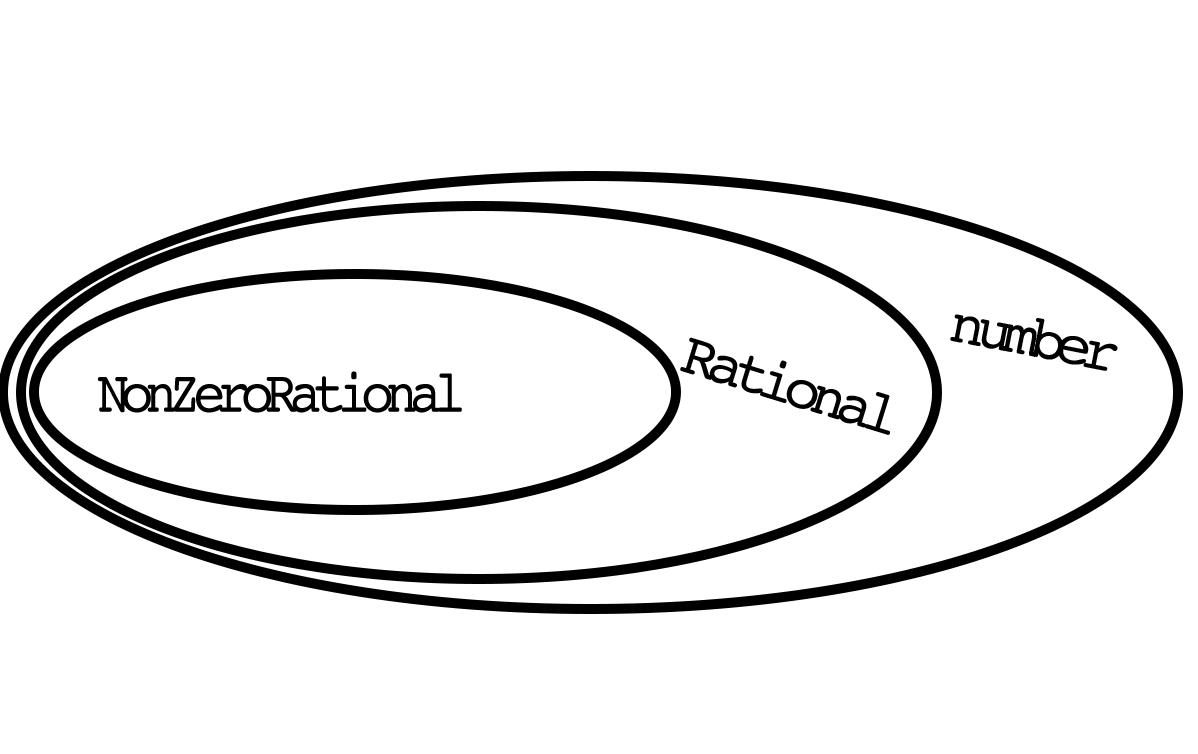
\includegraphics[width=7.1cm]{set_esimerkki}}
    \caption{Joukot NonZero, Rational ja number esitettynä osajoukkoina}
    \label{fig:set-esimerkki}
\end{figure}


Jos jakamisesimerkkiin määritetään joukot funktion argumenttien oikeiksi rajoitteiksi, ei funktiota voi käyttää väärin. TypeScript ei anna ajaa koodia, jos arvojen ei ole varmistettu kuuluvan oikeisiin joukkoihin (Koodiesimerkki \ref{code:ts_set_theory_6}) \cite{typsecript_website}.

\begin{code}
    \begin{minted}{typescript}
const divide = (x: Rational) => (y: NonZero) => x / y as Rational
\end{minted}
    \caption{Korrekti versio. Funktiolle annettavat arvot on varmistettava kuuluvan oikeisiin joukkoihin jossain vaiheessa ennen funktioon syöttöä käyttäen määriteltyjä \mintinline{javascript}|isRational| ja \mintinline{javascript}|isNonZero| funktioita }
    \label{code:ts_set_theory_6}
\end{code}

Aiempaan esimerkkiin voisi päätyä vaikkei olisi koskaan kuullut joukko-opista. Päällimmäisenä ajatuksena on kuitenkin se, että jos syötteitä ja palautusarvoja miettii joukkojen kannalta, syntyy luotettavampaa ohjelmakoodia ja vähemmän yllätyksiä. Tyypit ovat jo itsessään joukkoja, mutta niiden yksityiskohdat riippuvat käytössä olevasta, esimerkiksi ohjelmointikielen, tyyppijärjestelmästä \cite{type_theory}. Siksi ajatuksen tasolla joukkojen ajattelu on hyödyllistä.

Argumentit ja palautusarvot (tyypit) voi tietysti mieltää joukkoina myös \glsdisp{composed_function}{yhdistetyissä funktioissa} (Kuva \ref{fig:function_composition_in_sets}). Vaikka ohjelmoinnissa joukko-oppia ei rinnasteta ainoastaan funktionaaliseen ohjelmointiin,  joukko-opin ajattelu on siinä vähintäänkin tervetullutta.

\begin{figure}[htbp]
    \centering
    \begin{tikzpicture}
        % Ellipses for sets A, B, and C with background colors
        \draw[thick, ellipse, fill=green!20] (0,0.875) ellipse (0.8cm and 1.75cm);  % Set A with light blue background
        \draw[thick, ellipse, fill=blue!20] (3,0.875) ellipse (0.8cm and 1.75cm); % Set B with light green background
        \draw[thick, ellipse, fill=red!20] (6,0.875) ellipse (0.8cm and 1.75cm);   % Set C with light red background

        % Nodes for set A (without borders)
        \node[draw=none] (A1) at (0,2) {1};
        \node[draw=none] (A2) at (0,1.25) {2};
        \node[draw=none] (A3) at (0,0.5) {3};
        \node[draw=none] (A4) at (0,-0.25) {4};

        % Nodes for set B (without borders)
        \node[draw=none] (B1) at (3,2) {A};
        \node[draw=none] (B2) at (3,1.25) {B};
        \node[draw=none] (B3) at (3,0.5) {C};
        \node[draw=none] (B4) at (3,-0.25) {D};

        % Nodes for set C (without borders)
        \node[draw=none] (C1) at (6,2) {$\alpha$};
        \node[draw=none] (C2) at (6,1.25) {$\beta$};
        \node[draw=none] (C3) at (6,0.5) {$\gamma$};
        \node[draw=none] (C4) at (6,-0.25) {$\delta$};

        % Arrows from A to B
        \draw[->] (A1) -- (B1);
        \draw[->] (A2) -- (B3);
        \draw[->] (A3) -- (B2);
        \draw[->] (A4) -- (B4);

        % Arrows from B to C
        \draw[->] (B1) -- (C2);
        \draw[->] (B2) -- (C1);
        \draw[->] (B3) -- (C3);
        \draw[->] (B4) -- (C4);

        % Labels for sets
        \node[draw=none, text=green!50!black] at (-.5,3.25) {$A = \{1,2,3,4\}$};
        \node[draw=none, text=blue] at (3,3.25) {$B = \{A,B,C,D\}$};
        \node[draw=none, text=red] at (6.5,3.25) {$C = \{\alpha, \beta, \gamma, \delta\}$};

        % Arrow to new diagram
        \draw[->, line width=1.5mm, black] (3,-1.25) -- (3,-2.25) node[midway, right] {};

        % Corrected ellipses for sets A and C below the original picture
        \draw[thick, ellipse, fill=green!20] (0,-4.125) ellipse (0.8cm and 1.75cm);  % Set A with light blue background
        \draw[thick, ellipse, fill=red!20] (6,-4.125) ellipse (0.8cm and 1.75cm);   % Set C with light red background

        % Corrected nodes for set A (without borders) - Lower position
        \node[draw=none] (A1b) at (0,-3) {1};
        \node[draw=none] (A2b) at (0,-3.75) {2};
        \node[draw=none] (A3b) at (0,-4.5) {3};
        \node[draw=none] (A4b) at (0,-5.25) {4};

        % Corrected nodes for set C (without borders) - Lower position
        \node[draw=none] (C1b) at (6,-3) {$\alpha$};
        \node[draw=none] (C2b) at (6,-3.75) {$\beta$};
        \node[draw=none] (C3b) at (6,-4.5) {$\gamma$};
        \node[draw=none] (C4b) at (6,-5.25) {$\delta$};

        % Direct arrows from A to C (composition)
        \draw[->] (A1b) -- (C2b);
        \draw[->] (A2b) -- (C3b);
        \draw[->] (A3b) -- (C1b);
        \draw[->] (A4b) -- (C4b);
    \end{tikzpicture}
    \vspace{10pt}
    \caption{Funktioiden yhdistäminen joukko-opin näkökulmasta. Funktiot A$\,\to\,$B ja B$\,\to\,$C yhdistämällä saadaan A$\,\to\,$C. Älykkäällä kääntäjällä voi poistaa turhia laskutoimituksia. Keskimmäisen joukon evaluointi on käytännössä turhaa, jos funktiot ovat puhtaita}
    \label{fig:function_composition_in_sets}
\end{figure}


\subsection{Kategoriateoria}


Joukko-oppi ei ole ainoa ohjelmointiin sovellettava matemaattinen osa-alue. Funktionaaliselle ohjelmoinnille oleellisin osa-alue on \gls{category_theory} \cite{bartosz_category_for_progamers,promises-spec-94,dear_functional_bros}.

Kategoriateoria tutkii matemaattisia rakenteita ja niiden välisiä suhteita erittäin abstraktilla tasolla. Se keskittyy objektien (kuten joukkojen tai tyyppien) ja niiden välillä olevien morfismien (funktioiden tai muunnosten) tutkimiseen. Kategoriateorian avulla voidaan ymmärtää ja formalisoida monimutkaisia matemaattisia ja ohjelmallisia rakenteita. \citep{bartosz_category_for_progamers,promises-spec-94,category_theory}

Kategoriateoria on koettu ohjelmoijille erityisen mieluisaksi matematiikan haaraksi. Olisi algebra tai kalkyyli ohjelmoijalle jo ajatuksena hirveää, kategoriateorian on koettu olevan ohjelmoijille erityisen mieluisaa laajasta teoreettisuudesta huolimatta. \cite[9]{milewski2017category}.

Kategoriateoria näkyy jopa osittain myös nykypäivän JavaScriptissä, jossa Promise-tietorakenne toimii lähes kuin \gls{monad}. Promise-tietorakenne mahdollistaa asynkronisten operaatioiden ketjuttamisen ja virheiden käsittelyn tavalla, joka on verrattavissa kategoriateorian monadien tarjoamaan rakenteeseen. \citep{promises-spec-94,stackoverflow:why_monad}

Kategoriateoriaa ei käsitellä tässä opinnäytetyössä paljoa, sillä kirjoittaja ei tunne taitavansa sitä sellaisella tasolla, jolla voisi tiivistää tärkeimmät asiat oikealle tasolle. Ei myöskään nähdä hyötyä tuoda vaikeuttavaa tekijää sekoittamaan pakkaa.

Kategoriateoria on kuitenkin niin kytköksissä funktionaaliseen ohjelmointiin, ettei sitä voinut jättää kokonaan mainitsematta. Kategoriateorialle on kaivattu käytännönläheisempää tapaa lähestyä sitä ohjelmoijan näkökulmasta \cite{holvikari2021category}. Toisaalta on myös huomattu, että ohjelmoitaessa funktionaalista ohjelmointia puhtaasti, kategoriateorian oppii automaattisesti työn ohessa ilman tiukkaa teorian opiskelua \cite{holvikari2021category}.

\section{Tyyppijärjestelmät - tod.näk. rajaan ulos}

TODO

Tässä osassa voisi käydä läpi sitä, mitkä ovat ohjelmointikielen vaatimukset, että joukko-oppi-osan tyylistä koodia voi kirjoittaa. Tai missä roolissa tyyppijärjestelmät ovat funktionaalisessa ohjelmoinnissa (suuressa!).

Algebralliset tietorakenteet, joita eri tyyppijärjestelmät tukevat, on tosi isossa roolissa funktionaalisessa ohjelmoinnissa. Toisaalta ehkei ole pragmaattista jauhaa niistä.


% Tyypitys on todella tärkeää. Tyypit ohjaavat koodia ja estävät vääriä tiloja ohjemakoodin kääntämisvaiheessa. Tyypeillä pidetään ohjelmoija niissä raameissa, mitä funktionaalinen ohjelmointi usein vaatii \cite[44]{cantarella_fp_haitat}.

% JavaScriptissä tyypit eivät näy ohjelmoijalle muuten kuin sillon, kun ohjelma räjähtää ajon aikana. TypeScriptissä tyypit tulevat tielle. Haskelissa (ja PHP:ssa)

% \subsection{Staattinen ja dynaaminen tyypitys - todnäk rajaan ulos}

% \subsection{Nimellinen ja rakenteellinen tyypitys - todnäk rajaan ulos}

% \subsection{Parametrinen polymorfismi - todnäk rajaan ulos}

% Haskelille ominaista, fp ominaista.

% \subsection{Hindley-Milner tyyppijärjestelmä - todnäk rajaan ulos}

% Feldmanin mukaan, mahdottomat tilat ovat testausta parempaa \cite{impossiblebetter}.

% Myös Dijkstran idis abstraktiosta sopii kauniisti tähän, ja esimerkki siitä et mitä fp on parhaimmillaan.

% Parametrinen polymorfismi näkyy täs myös.


\section{Pragmaattisuus}

Funktionaalisen ohjelmoinnin tärkein teoria alkaa olla käytynä. On aika tarkastella teoreettisella tasolla sitä, miten funktionaalinen ohjelmoinnin voi tuoda \gls{js} (ja \gls{ts}) arsenaaliin.

Kun funktionaalisen ohjelmoinnin kauneus on matemaattisissa kulmakivissä, joilla ei ole tapaa taipua, miten sen voi yhdistää säännöttömään JavaScriptiin tai muuhun vastaavanlaiseen kieleen?

Mikä on se lähestymistapa, jota tarvitaan käytännönläheiseen, pragmaattiseen, funktionaaliseen ohjelmointiin?

\subsection{Monadi on monoidi endofunktorien kategoriassa}

Monadi on monoidi endofunktorien kategoriassa on fraasi, jota käytetään humoristisesti yhteyksissä, missä pyritään selittämään funktionaalisen ohjelmoinnin matemaattisen osa-alueen kategoriateorian \gls{monad}rakennetta \cite{bartosz_category_for_progamers_10}. Fraasi on surullisenkuuluisa, ja lienee yksi syy sille, miksei funktionaalinen ohjelmointi ole suositumpaa. Jos funktionaalisen ohjelmoinnin käsitteiden ymmärtämiseen tarvitsee useiden yliopistotasoisien kurssien taustatiedot, ei sopeutuminen ole helppoa.

Myöskin ohjelmoijat, jotka ovat tehneet kauan olio-ohjelmointia tai proseduraalista ohjelmointia, tahtovat toimia niillä tavoilla, mitä ovat oppineet. Esimerkiksi perustellaan niin, että JavaScript ei ole funktionaalinen ohjelmointikieli, vaikka siinä periaatteessa funktionaalista ohjelmointia voi kirjoittaakin. Tällaiset ongelmat tietysti ulottuvat pidemmälle kuin vain ohjelmointityyleihin. \citep{is_reduce_bad}

On harmillista perustella asioita pelkästään historiallisista syistä. Silloin ohjelmointikielet jäävät paikalleen \cite{promises-spec-94}.

\subsection{Funktionaalisen ohjelmoinnin ripottelu}

Kokemusten perusteella työpaikalla on havaittu funktionaalisen ohjelmoinnin paikallisuuden toimivan kohtuullisen hyvin muuten proseduraalisen ohjelmakoodin ympäristössä.

Robert C. Martinin mukaan pragmaattinen funktionaalinen ohjelmointi on sitä, että käytetään esimerkiksi \glsdisp{immutable_data}{muuttumattomuutta} ja puhtaita funktioita silloin, kun ne parantavat ohjelman luettavuutta, ylläpidettävyyttä ja suorituskykyä, ja kuitenkin niin, ettei vaadita täydellistä sitoutumista funktionaalisen ohjelmoinnin paradigmaan. \citep{martin2017pragmaticfp}

Myös Cantarella mainitsee opinnäytetyönsä loppupuolella ajatuksen, että mitä enemmän paradigmoihin liittyviin artikkeleihin perehtyy, sitä myötämielisemmäksi tulee ajatukselle, että paradigmoja tulisi yhdistellä vapaammin. \citep[45]{cantarella_fp_haitat}

Pragmaattista funktionaalista ohjelmointia vaikuttaa siis olevan se, että otetaan vain mitä tarvitaan \cite{dear_functional_bros,martin2017pragmaticfp,cantarella_fp_haitat}. Toisaalta se, mitä tarvitaan ei ole välittömästi selvää. Toisille pragmaattista on jättää kaikki matemaattinen teoria pois ohjelmoinnista heti kättelyssä, toisille kategoriateorian rakenteiden käyttäminen, kun niiden käyttäminen sopii ongelmaan \cite{holvikari2021category,martin2017pragmaticfp}.

\section{Funktionaalinen ohjelmointi \& TypeScript}
JavaScript ei ole funktionaalinen ohjelmointikieli, vaikka se funktionaalisuutta tukeekin \cite{is_reduce_bad}. TypeScriptin tyyppijärjestelmällä funktionaalinen ohjelmointi on jo mieluisampaa \cite{holvikari2021category}.


\subsection{Kielen sopivuus funktionaaliseen ohjelmointiin}

Vaikka TypeScript ei ole pohjimmiltaan funktionaalinen ohjelmointikieli, on sillä ominaisuuksia, joilla funktionaalisesta ohjelmoinnista tulee verraten helppoa.

TypeScriptissä on käytännössä kolme eri tapaa määrittää funktioita (Esimerkkikoodi \ref{code:javascript_function_types}). Nuolifunktioilla voidaan harjoittaa funktionaaliselle ohjelmoinnille tyypillistä argumenttien yksi kerrallaan antamista.


\begin{code}
    \begin{minted}{typescript}
function rnd(min: number, max: number) { 
	return Math.floor(Math.random() * max) + min;
}
const rnd2 = (min, max) => Math.floor(Math.random() * max) + min;
const rnd3 = min => max => Math.floor(Math.random() * max) + min;
\end{minted}
    \caption{Kolme eri tapaa kirjoittaa funktio JavaScriptissä \cite{okhravi-g-discussion}. Funktiomäärittely, funktioilmaus ja osittain sovellettava funktioilmaus}
    \label{code:javascript_function_types}
\end{code}

Myös koska funktiot ovat JavaScriptissä ensiluokkaisia (toisin sanoen käyttäytyvät kuin muuttujat), niitä voidaan antaa argumentteina toisille funktioilla (Koodiesimerkki \ref{code:js_first_class}). Tämä mahdollistaa funktionaaliselle ohjelmoinnille tyypillisten \glsdisp{higher_order_function}{korkeamman asteiden funktioiden} luomisen, ja käyttämisen.

\begin{code}
    \begin{minted}{javascript}
function A()  { return "moi"; }
function B(f) { return f(); }
B(A) // "moi"
\end{minted}
    \caption{Funktioiden ensiluokkaisuus JavaScriptissä}
    \label{code:js_first_class}
\end{code}

Funktionaalisen ohjelmoinnin piireissä TypeScriptin tyyppijärjestelmää arvostetaan myös, sillä sillä voidaan rakentaa ainakin osittain algebrallisia datatyyppejä, jotka ovat puhtaissa funktionaalisissa ohjelmointikielissä läsnä \cite{holvikari2021category}.


\subsection{Tyypitys}
TODO:
-- tämä osa ehkä rajataan pois --
TypeScriptin tyypitys on funktionaaliselle ohjelmoinnille hyvä, sillä siinä on mahdollista luoda summa-, ja tulotyyppejä (sum and product types) \cite{holvikari2021category,hickey_maybe_not}
-- --
\subsection{Kirjastot}

Funktionaalista ohjelmointia on pyritty pitämään elossa erinäköisin kirjastoin, joissa hyväksikäytetään kielen ominaisuuksia, ja luodaan kirjastoja, joiden käyttäminen vaatii ohjelmoijalta täysin uuden syntaksin opettelemista JavaScript syntaksin lisäksi \cite{ramda,sanctuary,crocks,fpts}.

Kokemusten perusteella syntaksierot ovat todella hidastava tekijä. Ohjelmoijat olettavat ohjelmoivansa TypeScript-projektissa TypeScriptiä. Tai yleisemmin sanottuna: ohjelmoijat olettavat ohjelmoivansa sitä ohjelmointikieltä mitä ohjelmoivat.

Funktionaalisen ohjelmoinnin kirjastoilla halutaan tuoda \gls{ts}-ekosysteemiin sitä, mitä siitä puuttuu. Kuitenkin on kirjasto kuinka hyvälaatuinen tahansa, tulee TypeScriptin tyyppijärjestelmä lopulta vastaan \cite{holvikari2021category}.



\subsection{Promise-tietorakenne ja osittaismonadisuus}

JavaScript on kielenä siitä erikoinen, että kaikki uusien versioiden ominaisuudet tulee olla takaperin yhteensopivaa. Jos tästä poikettaisiin, suuret määrät vanhoja verkkosivuja lakkaisivat toimimasta, sillä ne käyttäjät JavaScriptiä, ja odottavat sen toimivan vanhalla tutulla tavalla \cite{prototype_library_trends}.

Selaimille on myös parempi olla rikkomatta näitä vanhoja sivuja selaimen suosion kannalta: jos vierailee lääkärin vastaanoton verkkosivulla selvittääksesi aukioloajat, kumpi selain on paras: se, joka näyttää vastaanoton aukioloajat, vai se, joka ei näytä mitään, koska on ottanut uuden JavaScript-version käyttöön? \citep{against_self_closing_tags,proposal-joint-iteration}

Noin kymmenen vuotta sitten oli suuri keskustelu siitä, tulisiko JavaScriptin Promise-tietorakenteen noudattaa funktionaalisen ohjelmoinnin \glsdisp{monad}{monadirakennetta}. Tälle oli suuret perusteet, sillä rakenteen noudattaminen olisi vaatinut vain pieniä muutoksia ehdotettuun tietorakenteen toteutukseen \cite{promises-spec-94}. Perustelut monadin puolesta eivät kuitenkaan iskeneet lävitse muun muassa erinäisten väärinymmärrysten takia.

Monadin läsnäolo kielessä olisi mahdollistanut kielen viennin funktionaalisempaan suuntaan. Ja koska ohjelmointikielelle on tärkeää olla johdonmukainen, on erittäin epätodennäköistä, että kieli tulee saamaan enää koskaan toista mahdollisuutta tuoda monadia osaksi kielen ominaisuuksia \cite{proposal-joint-iteration,prototype_library_trends}.

Promise-tietorakenne on nykypäivänä erittäin vahvassa roolissa ohjelmoitaessa JavaScriptiä. Jos maailmassa olisi seurattu vaihtoehtoista historiaa, kieli saattaisi tänä päivänä tukea monia vastaavanlaisia ja standardoidulla tavalla toimivia tietorakenteita \cite{promises-spec-94}.
\section{Ramda.js}

TODO - Tätä tullaan käyttämään, mutta toisaalta ei ehkä relevanttia jauhaa turhaan. Muitakin kirjastoja saatetaan käyttää.


% Koska funktionaalisen ohjelmakoodin tuottaminen \gls{js} tai \gls{ts} ympäristössä enemmän tai vähemmän vaatii jotain kirjastoa, joko itse ohjelmoitua tai ulkoista, niin tähän insinöörityöhön on kirjastoksi valittu Ramda.js.

% Ramda.js, ja kirjaston taustalla oleelinen Fantasy Land -algebrallinen spesifikaatio, ovat kirjastoja jotka pyrkivät johdonmukaiseen funktionaaliseen ohjelmointiin JavaScriptissä. Näiden kirjastojen kehittäjistöstä löytyy samoja henkilöitä jotka aikoinaan pyrkivät saamaan Promise-tietorakenteen virallisesti monadiseksi \cite{ramda:contributors,fantasy-land:contributors,promises-spec-94}. Näyttää siltä, että kun tähän tavoitteeseen ei päästy, päättivät kehittäjät tuoda funktionaalisen ohjelmoinnin JavaScriptiin omin keinoin.

% miten ramda toimii

% miten ramda sopii omien funktioiden kanssa

% miten typescript? ei hyvä, tyypit ovat mitä sattuu (kokemuspohjaisesti)
